\documentclass[preprint,12pt,aps,pra,showkeys,amsmath,amssymb,superscriptaddress,floatfix]{revtex4-2}
\usepackage[T1]{fontenc}
\usepackage[utf8]{inputenc}
\usepackage{amsmath,amssymb,amsthm,mathtools,mathrsfs}
\usepackage{microtype,booktabs,enumitem}
\usepackage{xcolor,tikz,etoolbox}
\usepackage[skins,breakable]{tcolorbox}
\usepackage{needspace}
% Keep diagram geometry independent of REVTeX preprint body spacing.
\AtBeginEnvironment{tikzpicture}{\linespread{1}\selectfont}
\usetikzlibrary{arrows.meta,positioning,calc,fit,decorations.pathreplacing}
\usepackage{graphicx}
\usepackage{hyperref}

\definecolor{MMBlue}{RGB}{0,82,155}
\definecolor{MMOrange}{RGB}{200,80,0}
\tikzset{
 mmnode/.style={draw=MMBlue,rounded corners=2pt,fill=MMBlue!4,align=left,execute at begin node={\raggedright},text width=5cm,font=\fontsize{10}{12}\selectfont,inner sep=6pt},
 mmimport/.style={mmnode,draw=black!65,fill=black!4},
 mmcandidate/.style={mmnode,draw=MMOrange,dashed,fill=MMOrange!5},
 mmrejected/.style={mmnode,draw=black,densely dotted,fill=black!8},
 mmproof/.style={->,thick,MMBlue},
 mmflow/.style={->,semithick,black!70},
 mmrepair/.style={->,dashed,thick,MMOrange},
 mmcandidatearrow/.style={->,dashed,semithick,MMOrange},
 mmnote/.style={font=\scriptsize,fill=white,inner sep=2pt,align=center}}

\usepackage[section]{placeins}
\setlength{\emergencystretch}{3em}
\setlist{itemsep=3pt,topsep=4pt}
\newtheorem{theorem}{Theorem}[section]
\newtheorem{proposition}[theorem]{Proposition}
\newtheorem{lemma}[theorem]{Lemma}
\newtheorem{corollary}[theorem]{Corollary}
\theoremstyle{definition}
\newtheorem{definition}[theorem]{Definition}
\newtheorem{example}[theorem]{Example}
\theoremstyle{remark}
\newtheorem{remark}[theorem]{Remark}
% Avoid isolated statement headings and single-line paragraph fragments.
\BeforeBeginEnvironment{theorem}{\Needspace{6\baselineskip}}
\BeforeBeginEnvironment{definition}{\Needspace{5\baselineskip}}
\BeforeBeginEnvironment{proposition}{\Needspace{5\baselineskip}}
\BeforeBeginEnvironment{lemma}{\Needspace{5\baselineskip}}
\BeforeBeginEnvironment{corollary}{\Needspace{5\baselineskip}}
\clubpenalty=5000
\widowpenalty=5000
\newcommand{\R}{\mathbb R}\newcommand{\Z}{\mathbb Z}\newcommand{\N}{\mathbb N}
\newcommand{\Pa}{\operatorname{Pa}}\newcommand{\Desc}{\operatorname{Desc}}
\newcommand{\cl}{\operatorname{cl}}\newcommand{\cost}{\operatorname{cost}}
\newcommand{\status}{\operatorname{status}}
% Faculty cards: a visual rail groups the five faculties within one agent.
% The rail has no arrowhead and does not represent a proof dependency.
\newcommand{\mmfacultybadge}[1]{%
 \node[circle,draw=MMBlue,line width=1pt,fill=white,
 minimum size=7mm,inner sep=0pt,font=\sffamily\small\bfseries,text=MMBlue]
 at ([xshift=15pt,yshift=-15pt]frame.north west) {#1};}
\newcommand{\mmfacultyrail}{%
 \draw[MMBlue!80,line width=1pt]
 ([xshift=15pt,yshift=2pt]frame.north west)--
 ([xshift=15pt,yshift=-2pt]frame.south west);}
\newtcolorbox{mmfacultybox}[2]{enhanced,breakable,
 colback=MMBlue!4,colframe=MMBlue!4,boxrule=0pt,arc=3pt,
 left=39pt,right=9pt,top=4pt,bottom=4pt,
 before skip=2pt,after skip=2pt,
 fontupper=\small\linespread{1.1}\selectfont,
 overlay unbroken={\mmfacultyrail\mmfacultybadge{#1}},
 overlay first={\mmfacultyrail\mmfacultybadge{#1}},
 overlay middle={\mmfacultyrail},overlay last={\mmfacultyrail}}
\newcommand{\mmfaculty}[3]{%
 \begin{mmfacultybox}{#1}{#2}
 {\sffamily\bfseries\color{MMBlue}#2}\par\smallskip #3
 \end{mmfacultybox}}
\newcommand{\agent}[9]{%
 \Needspace{8\baselineskip}
 \subsubsection{#1}
 \noindent\textbf{Object.} #2\par
 \noindent\textbf{Role.} #3\par\smallskip
 \mmfaculty{E}{Ego}{#4}
 \mmfaculty{M}{Memory}{#5}
 \mmfaculty{I}{Intellect}{#6}
 \mmfaculty{S}{Sense}{#7}
 \mmfaculty{A}{Action}{#8}
 \smallskip\noindent #9\par}

\usepackage{longtable,array,calc}
\providecommand{\tightlist}{\setlength{\itemsep}{2pt}\setlength{\parskip}{0pt}}
\makeatletter
\def\frontmatter@abstract@produce{\par\addvspace{\frontmatter@preabstractspace}%
\begingroup\prep@absbox\unvbox\absbox\post@absbox\endgroup
\addvspace{\frontmatter@postabstractspace}}
\makeatother
\newcommand{\field}[2]{\par\smallskip\noindent\textbf{#1.} #2\par}
\setlength{\emergencystretch}{5em}
\AtBeginEnvironment{verbatim}{\small\linespread{1.0}\selectfont}


\hypersetup{colorlinks=true,linkcolor=MMBlue,urlcolor=MMBlue,pdfauthor={Dibakar Sigdel}}

\begin{document}

\title{Homology of the Torus\\[4pt]\large An End-to-End Meta-Math Walkthrough}

\author{Dibakar Sigdel}

\affiliation{Mindverse Computing LLC, Lynnwood, WA 98087, USA}

\date{October 2026}

\begin{abstract}

A complete authored walkthrough of homology of the torus, with explicit
mathematical contracts, local verification gates, and reusable exports.
The report presents the target theorem, declared imports, a dependency
graph, five-faculty node contracts, a continuous proof, a worked
example, and a hypothesis-repair audit. It is an authored mathematical
exposition, not a deployed-agent transcript or a formal proof-assistant
certificate.

\end{abstract}\maketitle\linespread{1.12}\selectfont

\noindent\textbf{AT-03 / Algebraic Topology / Report v1}

\section{Target and import contract}

\begin{theorem}

Compute integral homology of \(T^2\): \(H_0\cong\mathbb Z\),
\(H_1\cong\mathbb Z^2\), \(H_2\cong\mathbb Z\), and \(H_k=0\) for
\(k>2\).

\end{theorem}

\subsection{Foundations and permitted imports}

Use the square quotient CW structure on \(T^{2}\): one vertexv, oriented
edgesa,b, and one2-cellc attached alongaba \(^{-1}b^{-1}\). Import
cellular homology with integral coefficients: \(C_k\) is free on
k-cells, and its differential is the attaching-map incidence degree
after collapsing the other cells. Cellular homology agrees with singular
homology. AT-02 supplies this model; its \(\pi _{1}\) result is not
required for the boundary computation.

\clearpage\section{Node interaction workflow}

\begin{center}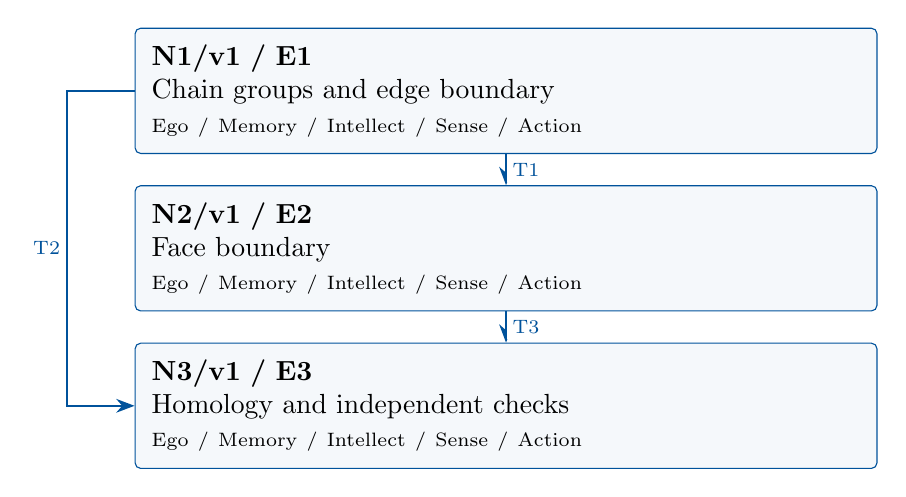
\begin{tikzpicture}[>=Stealth,x=1cm,y=1cm]

\node[mmnode,text width=9cm,minimum height=1.25cm] (N1) at (0,0.0) {\textbf{N1/v1 / E1}\\Chain groups and edge boundary\\{\scriptsize Ego / Memory / Intellect / Sense / Action}};

\node[mmnode,text width=9cm,minimum height=1.25cm] (N2) at (0,-2.0) {\textbf{N2/v1 / E2}\\Face boundary\\{\scriptsize Ego / Memory / Intellect / Sense / Action}};

\node[mmnode,text width=9cm,minimum height=1.25cm] (N3) at (0,-4.0) {\textbf{N3/v1 / E3}\\Homology and independent checks\\{\scriptsize Ego / Memory / Intellect / Sense / Action}};

\draw[mmproof] (N1.south) -- node[mmnote,right] {T1} (N2.north);

\draw[mmproof] (N1.west) -- (-5.58,0) -- node[mmnote,left] {T2} (-5.58,-4) -- (N3.west);

\draw[mmproof] (N2.south) -- node[mmnote,right] {T3} (N3.north);

\end{tikzpicture}\end{center}

Each box is one mathematical agent containing all five faculties. Blue
arrows carry the versioned exports listed below. The layout gives a
reading order; only drawn arrows assert dependencies. Diagnostic repair
is separate from the proof DAG.

\subsection{Versioned evidence-transfer ledger}

\begingroup\small\linespread{1.05}\selectfont

\Needspace{5\baselineskip}\field{T1: N1/E1/v1 to N2}{The chain groups and zero degree 1 differential.}

\field{Receiving activity}{N2: Face boundary}

\field{Compatibility}{Use the same mathematical objects and hypotheses as the source export.
Receiving contract: Attaching wordaba \(^{-1}b^{-1}\); prior exports
E1/v1}

\Needspace{5\baselineskip}\field{T2: N1/E1/v1 to N3}{The chain groups and zero degree 1 differential.}

\field{Receiving activity}{N3: Homology and independent checks}

\field{Compatibility}{Use the same mathematical objects and hypotheses as the source export.
Receiving contract: Both zero differentials; prior exports E1/v1, E2/v1}

\Needspace{5\baselineskip}\field{T3: N2/E2/v1 to N3}{The degree 2 differential is zero.}

\field{Receiving activity}{N3: Homology and independent checks}

\field{Compatibility}{Use the same mathematical objects and hypotheses as the source export.
Receiving contract: Both zero differentials; prior exports E1/v1, E2/v1}

\endgroup

\clearpage\section{Agent roles and five-faculty activities}\begingroup\small\linespread{1.05}\selectfont\setlist{itemsep=1pt,topsep=2pt}

\subsection{N1/v1: Chain groups and edge boundary}

\field{Object and role}{Count cells and compute endpoint incidences.}

\field{Inputs}{The CW cell model; foundational imports stated in §1}

\mmfaculty{E}{Ego}{Own E1/v1: The chain groups and zero degree 1 differential.}

\mmfaculty{M}{Memory}{Retain The CW cell model; foundational imports stated in §1; keep their
assumptions and versions attached.}

\mmfaculty{I}{Intellect}{Count cells and compute endpoint incidences.}

\mmfaculty{S}{Sense}{Identified endpoints still retain their opposite incidence signs.}

\mmfaculty{A}{Action}{Carry out the numbered deductions and publish E1/v1 together with its
hypotheses and proof location.}

\smallskip\noindent\textbf{Numbered mathematical activities}

\begin{enumerate}[label=N1.\arabic*,leftmargin=3.4em]

\item The cellular chain groups are \(C_{2}=Z\langle c\rangle\),
\(C_{1}=Z\langle a,b\rangle\), \(C_{0}=Z\langle v\rangle\) and zero in
higher degrees.

\item Both endpoints of each edge arev, with opposite endpoint signs, so
\(\partial _{1}a=v-v=0\) and \(\partial _{1}b=0\).

\end{enumerate}

\field{Export E1/v1}{The chain groups and zero degree 1 differential.}

\field{Acceptance gate}{Identified endpoints still retain their opposite incidence signs.
Publish only after checking every displayed deduction.}

\field{Targeted repair}{If the check fails, revise N1: Identified endpoints still retain their
opposite incidence signs. Recheck dependent nodes N2, N3.}

\clearpage

\subsection{N2/v1: Face boundary}

\field{Object and role}{Compute signed degree separately for each target edge.}

\field{Inputs}{Attaching wordaba \(^{-1}b^{-1}\); prior exports E1/v1}

\mmfaculty{E}{Ego}{Own E2/v1: The degree 2 differential is zero.}

\mmfaculty{M}{Memory}{Retain Attaching wordaba \(^{-1}b^{-1}\); prior exports E1/v1; keep
their assumptions and versions attached.}

\mmfaculty{I}{Intellect}{Compute signed degree separately for each target edge.}

\mmfaculty{S}{Sense}{Counting appearances without orientation would incorrectly produce2a+2b.}

\mmfaculty{A}{Action}{Carry out the numbered deductions and publish E2/v1 together with its
hypotheses and proof location.}

\smallskip\noindent\textbf{Numbered mathematical activities}

\begin{enumerate}[label=N2.\arabic*,leftmargin=3.4em]

\item Collapse all 1-cells excepta when computing the coefficient ofa in
\(\partial _{2}c\).

\item The attaching loop crossesa once forward and once backward, giving
degree \(1-1=0\).

\item The same calculation for b gives 0.

\item Therefore \(\partial _{2}c=0a+0b\).

\item This is a signed incidence computation, not an assumption that every
closed surface has zero cellular boundary in every chosen decomposition.

\end{enumerate}

\field{Export E2/v1}{The degree 2 differential is zero.}

\field{Acceptance gate}{Counting appearances without orientation would incorrectly produce2a+2b.
Publish only after checking every displayed deduction.}

\field{Targeted repair}{If the check fails, revise N2: Counting appearances without orientation
would incorrectly produce2a+2b. Recheck dependent nodes N3.}

\clearpage

\subsection{N3/v1: Homology and independent checks}

\field{Object and role}{Compute kernels modulo images in each degree.}

\field{Inputs}{Both zero differentials; prior exports E1/v1, E2/v1}

\mmfaculty{E}{Ego}{Own E3/v1: All integral homology groups in the target.}

\mmfaculty{M}{Memory}{Retain Both zero differentials; prior exports E1/v1, E2/v1; keep their
assumptions and versions attached.}

\mmfaculty{I}{Intellect}{Compute kernels modulo images in each degree.}

\mmfaculty{S}{Sense}{Euler characteristic alone cannot determine every homology group or its
torsion.}

\mmfaculty{A}{Action}{Carry out the numbered deductions and publish E3/v1 together with its
hypotheses and proof location.}

\smallskip\noindent\textbf{Numbered mathematical activities}

\begin{enumerate}[label=N3.\arabic*,leftmargin=3.4em]

\item The chain complex is \(0\to Z\to ^{0}Z^{2}\to ^{0}Z\to 0\), so
\(H_{2}=\operatorname{ker} \partial _{2}=Z\),
\(H_{1}=\operatorname{ker} \partial _{1}/\operatorname{im} \partial _{2}=Z^{2}\),
\(H_{0}=C_{0}/\operatorname{im} \partial _{1}=Z\), and \(H_k=0\) for
\(k>2\).

\item Its alternating rank sum \(1-2+1=0\) matches the cell count.

\item If independently using AT-02, \(H_{1}\) matches the abelianization of
\(\pi _{1}(T^{2})=Z^{2}\).

\item These checks support consistency but the kernel/image computation
establishes the groups.

\end{enumerate}

\field{Export E3/v1}{All integral homology groups in the target.}

\field{Acceptance gate}{Euler characteristic alone cannot determine every homology group or its
torsion. Publish only after checking every displayed deduction.}

\field{Targeted repair}{If the check fails, revise N3: Euler characteristic alone cannot
determine every homology group or its torsion. Withhold this terminal
result until its gate passes.}

\endgroup\clearpage\section{Continuous mathematical proof}\label{sec:proof}

Read these steps in order as one proof; the diagram is optional.
Numbered activities identify the specific constructions and deductions
owned by each node.

\subsection{§4.N1 --- Chain groups and edge
boundary}\label{n1-chain-groups-and-edge-boundary}

\begin{enumerate}
\def\labelenumi{\arabic{enumi}.}
\item
  The cellular chain groups are \(C_{2}=Z\langle c\rangle\),
  \(C_{1}=Z\langle a,b\rangle\), \(C_{0}=Z\langle v\rangle\) and zero in
  higher degrees.
\item
  Both endpoints of each edge arev, with opposite endpoint signs, so
  \(\partial _{1}a=v-v=0\) and \(\partial _{1}b=0\).
\end{enumerate}

\subsection{§4.N2 --- Face boundary}\label{n2-face-boundary}

\begin{enumerate}
\def\labelenumi{\arabic{enumi}.}
\item
  Collapse all 1-cells excepta when computing the coefficient ofa in
  \(\partial _{2}c\).
\item
  The attaching loop crossesa once forward and once backward, giving
  degree \(1-1=0\).
\item
  The same calculation for b gives 0.
\item
  Therefore \(\partial _{2}c=0a+0b\).
\item
  This is a signed incidence computation, not an assumption that every
  closed surface has zero cellular boundary in every chosen
  decomposition.
\end{enumerate}

\subsection{§4.N3 --- Homology and independent
checks}\label{n3-homology-and-independent-checks}

\begin{enumerate}
\def\labelenumi{\arabic{enumi}.}
\item
  The chain complex is \(0\to Z\to ^{0}Z^{2}\to ^{0}Z\to 0\), so
  \(H_{2}=\operatorname{ker} \partial _{2}=Z\),
  \(H_{1}=\operatorname{ker} \partial _{1}/\operatorname{im} \partial _{2}=Z^{2}\),
  \(H_{0}=C_{0}/\operatorname{im} \partial _{1}=Z\), and \(H_k=0\) for
  \(k>2\).
\item
  Its alternating rank sum \(1-2+1=0\) matches the cell count.
\item
  If independently using AT-02, \(H_{1}\) matches the abelianization of
  \(\pi _{1}(T^{2})=Z^{2}\).
\item
  These checks support consistency but the kernel/image computation
  establishes the groups.
\end{enumerate}

\hfill$\square$

\section{Worked orchestration}

The oriented2-cellc is a generator of \(H_{2}\) because its boundary is
0 and there are no3-cells to make it a boundary. The classesa,b
independently generateH \(_{1}\); an integer \(cycle3a-2b\) is nonzero
because \(\operatorname{im} \partial _{2}=0\).

\subsection{Boundary and hypothesis audit}

For \(RP^{2}\) the 2-cell attaches by a degree 2 loop, so
\(\partial _{2}\) is multiplication by 2 and \(H_{1}=Z/2\), \(H_{2}=0\).
Sense uses this comparison to reject the claim that all face boundaries
vanish merely because an attaching word is closed.

\section{Illustrative failure and repair}

The following is an authored diagnostic scenario. Changed assumptions
define a new contract; they do not retroactively prove the original
statement.

\subsection{Failure and correction}
This is an authored teaching trace, not a recorded agent run.

\begin{enumerate}
\def\labelenumi{\arabic{enumi}.}
\tightlist
\item
  \textbf{Ego \(\to\) Memory:} register the §1 theorem, imports, and
  requested exports before beginning the proof.
\item
  \textbf{Intellect \(\to\) Action:} choose the bridges in §3 and carry
  out the numbered activities in §4; transmit only established E-exports
  along the §2 DAG.
\item
  \textbf{Sense \(\to\) responsible node:} test the specific
  boundary/failure in §5 and the node's individual audit. A failing
  candidate is withheld; downstream nodes may not use it.
\item
  \textbf{Memory + Intellect:} identify whether the error is an omitted
  condition, an invalid inference, or an attempted extension beyond the
  theorem. Restore the exact contract or explicitly state a different
  one.
\item
  \textbf{Action:} redo the affected mathematical activity using the
  repaired condition or inference. Recheck consuming nodes, rather than
  feeding their conclusions back as premises.
\item
  \textbf{Ego:} publish only the supported export with its assumptions
  and proof location. A hypothetical revised export is v2; the written
  proof here is the v1 exposition, not a claim that this repair was
  executed.
\end{enumerate}

\subsection{Hypothesis boundary}
For \(RP^{2}\) the 2-cell attaches by a degree 2 loop, so
\(\partial _{2}\) is multiplication by 2 and \(H_{1}=Z/2\), \(H_{2}=0\).
Sense uses this comparison to reject the claim that all face boundaries
vanish merely because an attaching word is closed.

\subsection{Version and recheck}
Treat any changed assumption as a new contract. Recheck the revised
export and all of its descendants. A backward diagnostic never
establishes an earlier theorem. This is an authored teaching trace, not
an execution log.

\par\medskip\begingroup\small\linespread{1.0}\selectfont\noindent\textbf{Provenance.} This authored proof is complete relative to its declared imports. Reuse
each export with its assumptions, proof, and version. The original
Markdown remains available for comparison.
\par\endgroup

\par\smallskip\begingroup\small\linespread{1.0}\selectfont\noindent\textbf{Further reading.} \begin{itemize}
\tightlist
\item
  \href{https://pi.math.cornell.edu/~hatcher/AT/AT.pdf}{Allen Hatcher,
  Algebraic Topology: covering spaces, cellular homology, and cap
  products}.
\end{itemize}\par\endgroup

\end{document}
